\documentclass[a4paper,11pt]{article}

\usepackage{graphicx}
\usepackage{subfig,hyperref}


\begin{document}
\title{ML CS726 Fall'11 Project 2 Complex Classifiers}
\author{Angjoo Kanazawa, Ran Liu, Austin Myers}
\maketitle


\section{Gradient Descent and Linear Classification}
\subsection{WU1}
\textsf{Find a few values of step size where it converges and a few
  values where it diverges. Where does the threshold seem to be?}\\
It depends on what the number of iteration is, but with 100
iterations, from step 0.1 to 6.5 it finds a solution close to
0. But right after 6.6, it starts to diverge and for any value after
6.7 it diverges. The treshold seems to be around 6.6.

\subsection{WU2}
\textsf{Come up with a non-convex univariate optimization
  problem. Plot the function you're trying to minimize and show two
  runs of gd, one where it gets caught in a local minimum and one
  where it manages to make it to a global minimum. (Use different
  starting points to accomplish this.)}\\
Using $f(x) = sin(\pi x) + x^2/2$, $f'(x) = \pi cos(\pi x) + x$, and
10 iterations, the
global minimum happens at $x\approx -0.45385$.
If we start at 0, we can find the global minimum, but if we start at
1, gd gets caught in a local minimum $1.357$
Output:
\begin{verbatim}
>>> gd.gd(f, derF, 0, 10, 0.2)
(-0.45385351939658519, array([ 0 -0.72244765, -0.84494752, -0.88472033, -0.88650671,-0.88651822, -0.88651823, -0.88651823, -0.88651823, -0.88651823, -0.88651823]))
>>> gd.gd(f, derF, 1, 10, 0.2)
(1.3577434052579487, array([  1.22464680e-16, 4.52961014e-02,
2.50055080e-02, 2.00175811e-02, 1.99477186e-02, 1.99477147e-02,
1.99477147e-02, 1.99477147e-02, 1.99477147e-02, 1.99477147e-02, 1.99477147e-02]))
\end{verbatim}
The first run finds the global minimum, but the second one
doesn't. (the first value in the ouptut of gd is the solution it found)
\subsection{WU3}
\textsf{Why does the logistic classifier produce much larger weights
  than the others, even though they all get basically the same
  classification performance?}\\ Don't have to answer this.

\section{Warm Up with ML Tools}
\label{sec:warmup}
\subsection{WU4}
\textsf{What are the five features with largest positive weight and what
are the five features with largest negative weight? Do these seem "right"
based on the task?}\\

\begin{enumerate}
 \item motif -1.21427941322326660156
 \item window -1.15418136119842529297
 \item server -0.94833439588546752930
 \item list -0.89077484607696533203
 \item x -0.86568439006805419922
\end{enumerate}

\begin{enumerate}
 \item graphics 1.09135174751281738281
 \item images 0.72243607044219970703
 \item image 0.72001230716705322266
 \item card 0.71239823102951049805
 \item xx 0.69124054908752441406
\end{enumerate}

\subsection{WU5}
\textsf{ Draw the tree. How do the selected features compare to the
  features from the logistic regression model? Which features seem
  "better" and why? If you use a depth 10 tree, how well do you do on
  test data?}\\
\begin{figure}[h!]
  \caption{WU5: The tree}
  \centering
   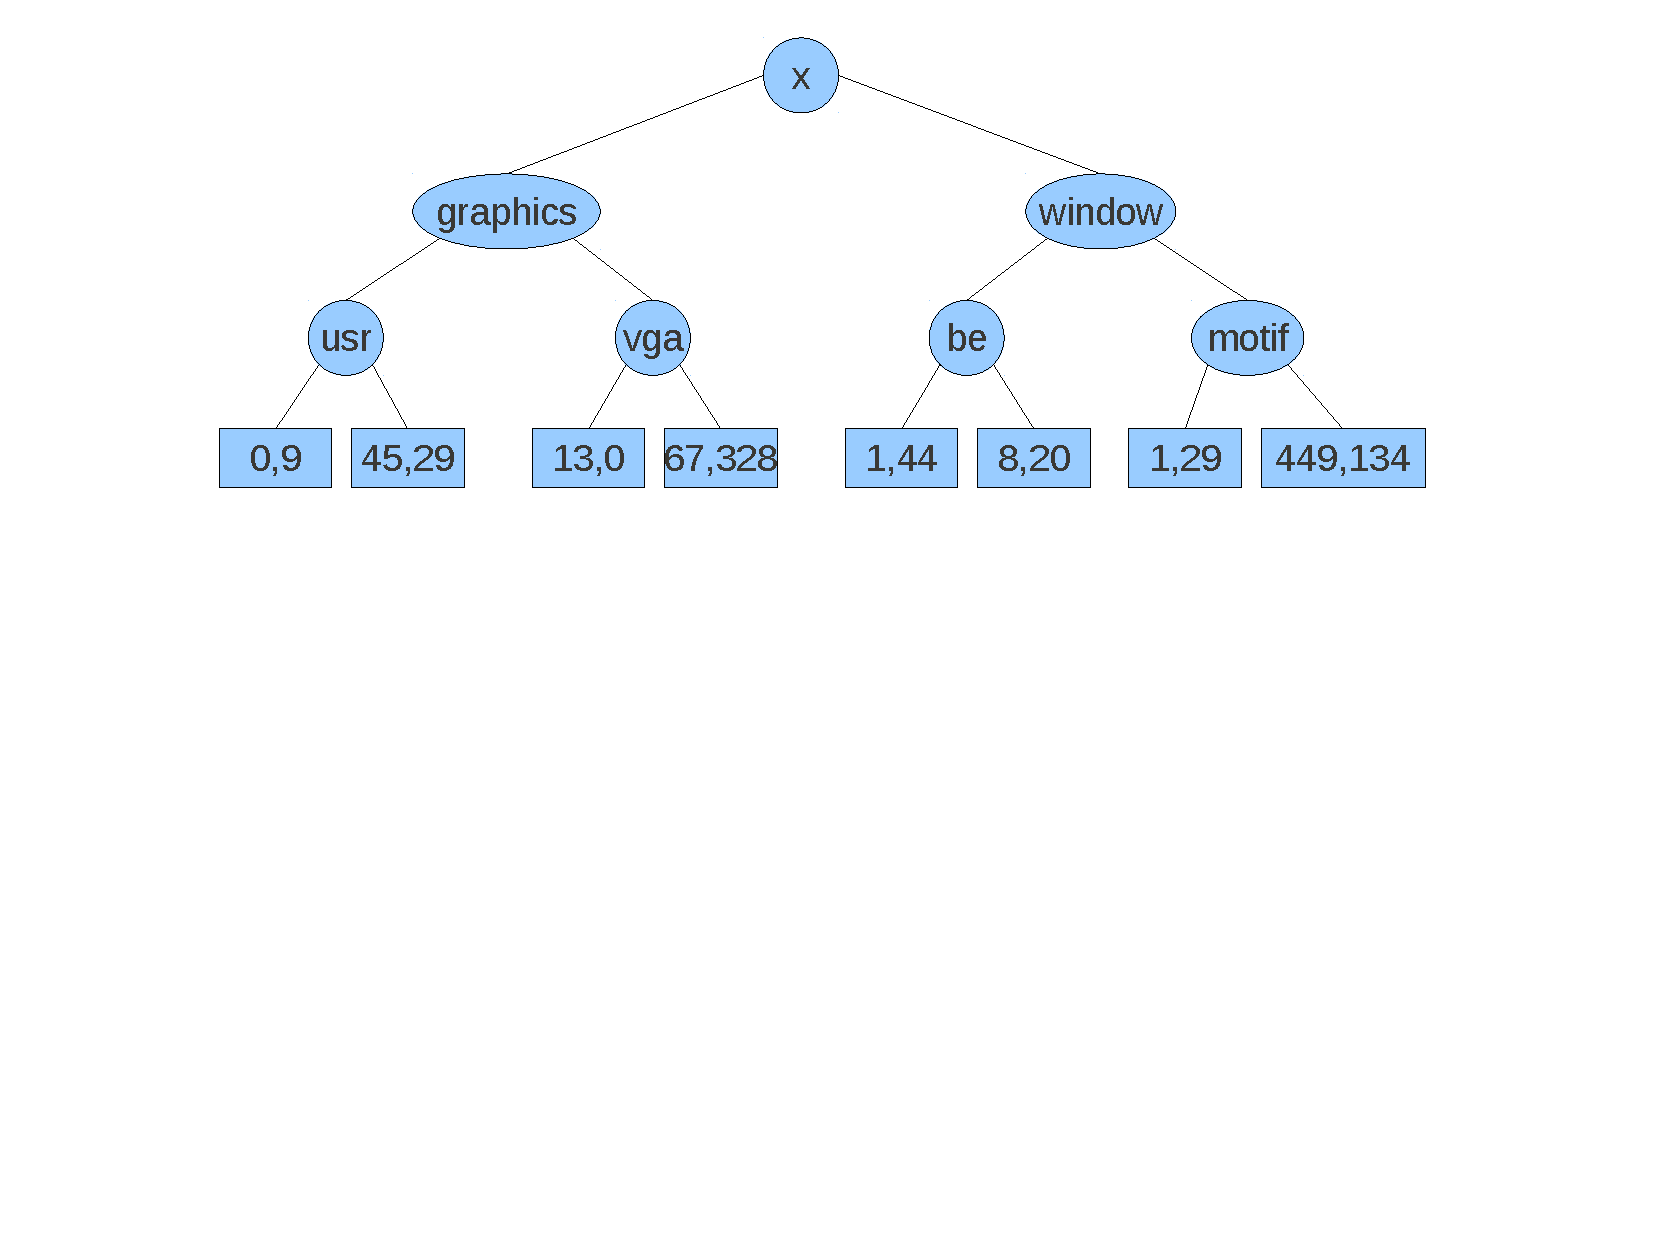
\includegraphics[width=5in]{wu5_tree.pdf}
\end{figure}

The selected features include four of the best/worst features from
the logistic regression (``graphics'', ``motif'', ``window'', and ``x'').

Features can be considered ``better'' when the ratio bewteen class 1
and class 0 at the leaf is higher and when the frequency of the number
of instances that got to that leaf is high. In this respect, ``motif''
and ``vga'' are the better features. ``motif'' has high frequency
(total 583 instances fall have no motif) and high ratio (about 80\% of
those without ``motif'' are in class 1).  395 instances fall in
``vga'', and 84\% of those with no ``vga'' are in class 0. If they
have ``vga'', 100\% of them are in class 1 (although this may not be the
best indicator because only 13 data falls into yes ``vga''.) 
In this respect, ``usr'' is one of the worst features in this tree
because the relative frequency is low, adn when there is no ``usr'',
the ratio of class1 to class0 is 6:4.

If I use a depth 10 tree, I get a test error of 20.53\%, (0.463\%
improvement).

\subsection{WU6}
\textsf{}\\

\subsection{WU7}
\textsf{}\\

\section{Reductions for Multiclass Classification}
\subsection{WU8}
\textsf{}\\

\subsection{WU9}
\textsf{}\\
\pagebreak
\subsection{Ranking or Collective Classification}
\subsection{WU10b}
\textsf{plot the accuracy of your classifier as a function
  of the number of levels in the stack. Do you observe that stacking
  helps? I.e., does some layer >1 perform better than layer 1? If not,
  perhaps you're not using sufficiently helpful features between the
  layers. Does the stack ever overfit? Plot your training error versus
  your test error as a function of the number of layers, and if you
  observe massive overfitting, you might need to do cross-validation
  to attenuate this. Report on your experience.}\\
We chose collective classification. 

We used the cora dataset (\url{www.research.whizbang.com/data}), which is a collection of
2708 Machine Learning papers. The papers are classified into one of the seven
classes (Case Based, Genetic Algorithms, Neural Networks,
Probabilistic Methods, Reinforcement Learning, Rule Learning,
Theory). The data is represented by 1433 unique words.
The cora dataset also comes with the citation graph of the papers
which we use as edges (links) between documents. There are total of
5429 directonal links.

For collective classification, the original feature we used was a
vector indicating the ID of the word in the vocabulary that is present
in the paper.

In each of the stacking process, for each document we counted how many
neighbors of the document were classified as each possible class,
normalized the counts, and added those values as new features. i.e. if
document A linked to document B, C, D, and E, which were classified as
class 4, 2 and 2, 3 respectively by the previous classifier, our new feature would add the
information that 50\% of A's neighbors were class 2, and 25\% class 4
and 3. 

We randomly selected 80\% of documents (2150) to use as training data
and the remaining 20\% as testing data (550).\\


Does stacking help?\\


Does the stack ever overfit? Figure 2 is the plot of our training
error versus your test error as a function of the number of layers.
\begin{figure}[h!]
  \caption{WU10b: Training error and test error as a fn of the number of layers }
  \centering
%   \includegraphics[width=5in]{WU5/traintest.png}
\end{figure}\\

We tried
\end{document}
